\documentclass[11pt,a4paper,notitlepage]{article}

\usepackage[margin=3cm]{geometry}

\usepackage{bookmark}

\usepackage{hyperref}
\hypersetup{colorlinks=true,urlcolor=blue,linkcolor=black}

\usepackage{enumitem}
\setlist[enumerate]{leftmargin=*}
\setlist[itemize]{leftmargin=*}

\usepackage{listings}
\lstset{
  basicstyle=\ttfamily,
  columns=flexible,
  escapechar=@,
  tabsize=4,
  commentstyle=\color{darkgray},
  frame=l,
  framerule=1pt}
\NewDocumentCommand{\mono}{m}{\lstinline{#1}}
\lstnewenvironment{code} {\lstset{language=C}} {}

\usepackage{calc}

\usepackage{float}

\usepackage{booktabs}

\usepackage{xcolor}

\setlength{\parindent}{0pt}
\setlength{\parskip}{.5em}
\setlength{\skip\footins}{2em}

\renewcommand*\familydefault{\sfdefault}

\usepackage{graphicx}
\graphicspath{{img/}}

\usepackage{tcolorbox}
\tcbset{parbox=false}
\newenvironment{infobox} {\begin{tcolorbox}[title=Info]} {\end{tcolorbox}}

\newcommand{\zephyrversion}[0]{3.5.0}
\newcommand{\sdkversion}[0]{0.16.3}
\newcommand{\imagename}[0]{zephyr\_stm32\_v\zephyrversion{}}
\newcommand{\cmdinwsl}[0]{wsl -d \imagename{}}

\newcommand{\maintitle}[0]{Zephyr Development Environment Container}

\NewDocumentCommand{\puttitle}{m}{%
  \begin{center}
    \huge
    \begin{minipage}[b]{.4\textwidth}
      
\includegraphics[height=2.5em]{en-zhaw-ines}
    \end{minipage}%
    \begin{minipage}[b]{.6\textwidth}
      \begin{flushright}
        \textbf{\maintitle}\\
        #1
      \end{flushright}
    \end{minipage}%
    \vspace{1cm}
  \end{center}
  \lfoot{\maintitle{} #1}
}

\usepackage{fancyhdr}
\pagestyle{fancy}
\lhead{}
\chead{}
\rhead{}
\lfoot{}
\lfoot{}
\cfoot{}
\rfoot{\thepage}
\renewcommand{\headrulewidth}{0pt}
\renewcommand{\footrulewidth}{0pt}


\begin{document}

\puttitle{}

\section{Introduction}

These instructions explain the setup of a containerized environment for
developing Zephyr applications. This environment can either be used with a
container runtime or the \emph{Windows Subsystem for Linux}.

The \emph{Containerfile} can be found in Appendix~\ref{containerfile} for anyone
interested.

\section{Technical Background (optional read)}

\subsection{Necessity for WSL or Containers}

In the following labs, you are going to work with the Zephyr RTOS. By providing
a containerized environment, we can ensure a reproducible setup. Additionally,
the images are lightweight, have a small memory footprint, and outperform a
conventional VM.

\subsection{Windows Subsystem for Linux}

The Windows Subsystem for Linux (WSL 2) is available for Windows 10/11 since
2019. Not all Windows Versions include it per default, an installation is
possible via the Microsoft Store or \emph{winget}. WSL 2 runs inside a managed
virtual machine (VM) that includes a Linux kernel. The virtualization is
implemented via a highly optimized subset of Hyper-V features. WSL 2 on Windows
11 can retain up to 95 \% of the performance of a native Linux Distribution.

\subsubsection*{Benefits compared to a conventional VM}

\begin{itemize}
\item Seamless integration in Windows. Files contained within the WSL can be
  accessed directly via the regular Windows file explorer.
\item After creating a WSL image, it can be started directly in the file explorer.
\item The VM setup is seamless and executed automatically without user
  interaction.
\end{itemize}

\subsection{Container Runtime}
Container runtimes are an alternative to the VM that WSL 2 provides. These
runtimes are typically developed for linux systems\footnote{Docker and Podman
  are available for Windows but run in WSL 2 in the background}. Two notable
container runtimes are \emph{Docker} and \emph{Podman}.

\newpage

\section{Setup with WSL}

Follow these steps to set up a Zephyr development environment in the WSL.

\begin{itemize}
  \item Install the \emph{J-Link Software and Documentation pack}.
        Make sure to tick the \emph{Install USB Driver for J-Link (requires admin rights)}
        checkbox during installation.

        \href{https://www.segger.com/downloads/jlink/JLink_Windows_x86_64.exe}{Download}

  \item Install \emph{PuTTY} or another application that can be used for serial
      communication. Either download from \href{https://putty.org/}{here} or
      install with \emph{winget}:

        \begin{lstlisting}
winget install --id PuTTY.PuTTY -e
\end{lstlisting}

  \item Optional: install \href{https://aka.ms/terminal}{\emph{Windows Terminal}}
      for a better terminal experience.

        \begin{lstlisting}
winget install --id Microsoft.WindowsTerminal -e
\end{lstlisting}

  \item Open a terminal.

  \item Ensure that the WSL is installed.
        \begin{lstlisting}
wsl --install --no-distribution
\end{lstlisting}

        \begin{infobox}
          After installing WSL, make sure to reboot your machine. Otherwise the changes
          will not be applied.
        \end{infobox}

        \begin{infobox}
          If you see the help output of \mono{wsl} try without the
          \mono{--no-distribution} switch. If you get an error try installing
          the WSL from the Windows Store. This can be done with in the
          \emph{Microsoft Store} or with \mono{winget}:
          \begin{lstlisting}
winget install "Windows Subsystem for Linux"
\end{lstlisting}
        \end{infobox}
  \item Create a folder for the environment and import the provided WSL image.
        \begin{lstlisting}
mkdir D:\wslDistroStorage\@\imagename{}@
wsl --import @\imagename{}@ `
  D:\wslDistroStorage\@\imagename{}@ `
  "$env:USERPROFILE\Downloads\@\imagename{}@_wsl.tar.gz"
\end{lstlisting}
  \item Open a shell inside the environment.

        \begin{lstlisting}
@\cmdinwsl{}@
\end{lstlisting}

        \begin{infobox}
          In case you get a \emph{CreateProcessParseCommon:789: Failed to
          translate D:\textbackslash} error the file system might not be
          available from within WSL. Run the following command to list the
          available file systems.

          % \cmdinwsl{ls /mnt}
          \begin{lstlisting}
@\cmdinwsl{}@ ls /mnt
\end{lstlisting}

          You can try mounting the missing file system
          (\mono{D:\\} in this case) with the following
          commands.

          \begin{lstlisting}
@\cmdinwsl{}@ mkdir /mnt/d
@\cmdinwsl{}@ mount -t drvfs D: /mnt/d
\end{lstlisting}
        \end{infobox}
        \begin{infobox}
          If you are using \emph{Windows Terminal} you can conveniently open a
          new tab with the environment. You might have to restart the terminal
          for this option to appear.
          \begin{center}
            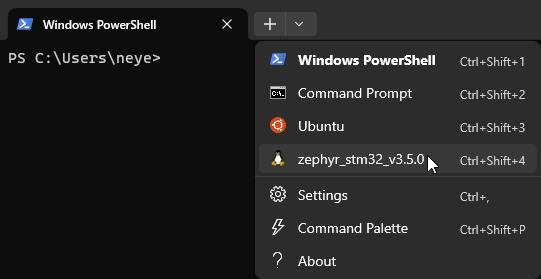
\includegraphics[width=.5\paperwidth]{terminal_open_wsl_tab}
          \end{center}
        \end{infobox}
\end{itemize}

\newpage

\section{Setup with a Container Runtime}

\begin{itemize}
  \item Install the \emph{J-Link Software and Documentation pack
        (\href{https://www.segger.com/downloads/jlink}{Download})}.
  \item Install a serial terminal like \mono{minicom}.
  \item Install a container runtime (e.g. \emph{podman} or \emph{docker}).
  \item Load the image.
        \begin{lstlisting}
podman load --input @\imagename{}@.tar.gz
\end{lstlisting}
  \item Run the container.
        \begin{lstlisting}
podman run --rm -it \
  -v /path/to/project:/root/dev \
  @\imagename{}@
\end{lstlisting}
\end{itemize}

\newpage

\section{Using the Zephyr Environment}

\subsection{Build Sample}

Run the following inside the environment to compile the blinky sample.

\begin{lstlisting}
cd ~/zephyrproject/zephyr/samples/basic/blinky/
west build --pristine --board stm32f429i_disc1 --build-dir /tmp/build
\end{lstlisting}

% container runtime: make sure builddir accessible

\subsection{Flash Sample}

Start \emph{J-Flash Lite} and select the target device (\mcutype{}). In the next
window select the firmware file (\mono{build/zephyr/zephyr.hex}) and click on
\emph{Program Device}.

% \begin{center}
%   \includegraphics[width=.5\paperwidth]{jflashlite_1.png}
% \end{center}

\begin{infobox}
  The WSL file system can be accessed in the explorer.
  \begin{center}
    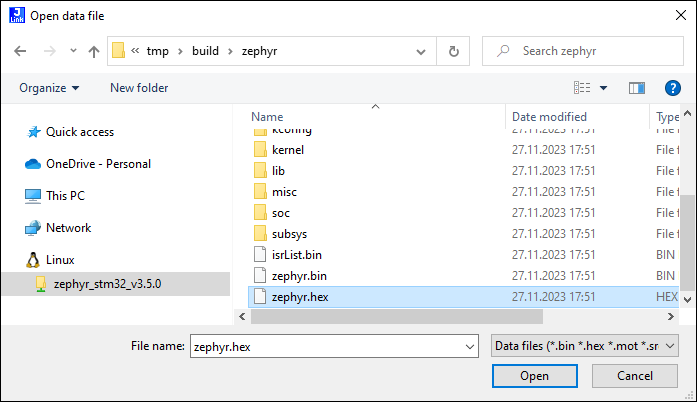
\includegraphics[width=.5\paperwidth]{explorer_wsl_hex}
  \end{center}
\end{infobox}

See Appendix~\ref{jlinkremote} for an alternative solution where \mono{west
flash} can be used to flash the target.

Open a serial terminal with e.g. PuTTY to see the log output:

\begin{lstlisting}
plink.exe -sercfg 115200 -serial com3
\end{lstlisting}

You might have to press the reset button on your microcontroller board to start
the program and print the message again.

\begin{infobox}
  Open the device manager to find the COM-port number.
  \begin{center}
    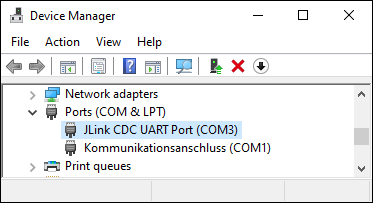
\includegraphics[width=.5\paperwidth]{device_manager_com}
  \end{center}
\end{infobox}

\newpage

\appendix

\section{Alternative to J-Flash Lite}\label{jlinkremote}

The \emph{J-Link Remote Server} can be used to flash from within the container.
Start the J-Link Remote Server on the host now.

\begin{infobox}
  If the J-Link Remote Server shows an error try using a different port (19020
  is the default).
\end{infobox}

Run the following command in a PowerShell to get the IP of the WSL network
adapter.

\begin{lstlisting}
@\cmdinwsl{}@ grep nameserver /etc/resolv.conf
\end{lstlisting}

Then run the following command to flash the board (replace the IP with the one
from above).

\begin{lstlisting}
west -v flash --runner jlink \
  --tool-opt='-ip 172.21.160.1:19020' \
  --build-dir /tmp/build
\end{lstlisting}

\begin{infobox}
  On Linux, add the \mono{--network="host"} argument to \mono{podman run}
  and use \emph{127.0.0.1} as the IP address.
\end{infobox}

\begin{infobox}
  If you get a \emph{FAILED: Can not connect to J-Link via TCP/IP} error try
  adding a firewall rule that allows inbound connections on the WSL network
  adapter. To do that, run the following command in an admin PowerShell.

  \begin{lstlisting}
New-NetFirewallRule -DisplayName "WSL" -Direction Inbound `
 -InterfaceAlias "vEthernet (WSL)" -Action Allow
\end{lstlisting}

  Firewall rules can also be managed by running \mono{wf.msc} in a PowerShell.
\end{infobox}

\newpage

\newgeometry{margin=2cm}
\fancyfoot{}

\section{Containerfile}\label{containerfile}

\lstinputlisting[basicstyle=\ttfamily\scriptsize]{../Containerfile}

Usage example:

\begin{lstlisting}
podman build \
  --build-arg="ZEPHYR_VERSION=@\zephyrversion@" \
  --build-arg="SDK_VERSION=@\sdkversion@" \
  . -t @\imagename@
\end{lstlisting}

\end{document}

% Local Variables:
% TeX-output-dir: "build"
% TeX-master: t
% End:
